\section{Object Recognition, Methods and Implementation}\label{sc:obj_final}
This section serves to describe how knowledge of objects can be represented and included in the previously mentioned recognition methods through classification of the object properties.

\subsection{Object Recognition}\label{ssc:object_recognition}
The previous sections have described how to detect edges, contours, borders and regions in an image, how this detection could be described for an analysis to happen, and how recognition could be done. The more detailed recognition methods were done with described properties, which only recognised one unique instance, that would need a good match.

Object recognition serves to extend the area of recognition, through pattern recognition which can be seen as a synonym to object recognition, the extension is done by expanding the concept of objects and performing a classification of the objects based on certain properties. Classifiers are used to perform this ordering and use a class of properties called sensed properties. Sensed properties cover characteristics such as texture, reflexive properties, and shape and does not cover properties like the molecular structure of the objects, which also would be impossible information to achieve with a normal camera. The sensed object defines patterns of the objects and it is these patterns that are recognised with object recognition. \Cref{fig:pat_recog} shows the steps that are taken in pattern recognition. The first block, \textit{Construction of formal description}, involves the designer and his experience and intuition with the object to be described. Through patterns that the designer specifies, the patterns can be defined and these con be used to create classifiers, which can classify objects.
\begin{figure}[H]\centering
  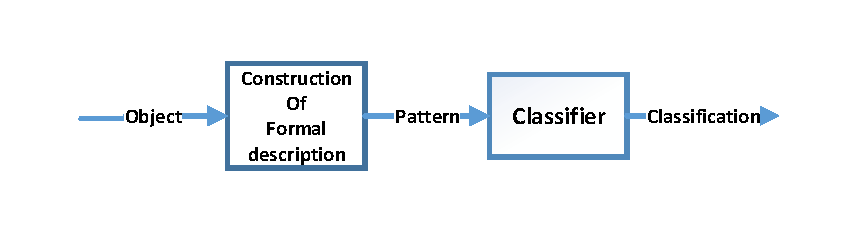
\includegraphics[width=0.8\textwidth]{graphics/pattern_recognition.pdf}
  \caption{Main pattern recognition steps \citep{obj_recogn_book}}
  \label{fig:pat_recog}
\end{figure}

It has been stated that no recognition can be done without some knowledge of the object to be recognised\citep[Page 381]{obj_recogn_book}. This knowledge is what specifies the properties that are to be recognised by the classifiers. Furthermore, the structure of how the knowledge is represented can be beneficial for how the pattern recognition is performed. In general pattern recognition is divided in two types; \textit{statistical} and \textit{syntactic}, which are described after knowledge representation is presented.\citep{obj_recogn_book}

\subsubsection{Knowledge Representation}\label{ssc:knowledge_representation}
There are many ways to represent the knowledge that is needed for pattern recognition and each representation can be used for any of the pattern recognition methods, however some representation methods are more beneficial for certain pattern recognitions, the two representations that are introduced here are mainly for statistical and syntactic recognition, respectively. 

\emph{Descriptions and features}

Even though descriptions are not considered pure knowledge representations, as they do not give a generalised representation, they can be used to represent some knowledge, as part of a greater, more complex structure \citep[Page 382]{obj_recogn_book}.
Features are representations of scalar properties, which can be used to describe object relations. To gather multiple descriptions for an object, \textit{feature vectors} are used. These feature vectors can in turn be used as input for statistical pattern recognition techniques.

An example of a feature vector can be of two features, \textit{compactness} (see \cref{ssc:heuristic_descr}), which can be used to determine the circularity of objects (perfectly round objects are the most compact), and a feature called \textit{size} which is used for describing the area of the given object. From these features a feature vector would be $x=(size, compactness)$. With definitions of what is small or big, and accepted circularity, the feature vector can then be used to classify objects as small, large, circular, non-circular and so forth.

\emph{Grammars and languages}

The description methods that were used to describe shapes, can also be used to describe objects. But to have the more general representation of an object class, these description methods are not sufficient. However, a way to classification is with the use of grammars and languages which is used in syntactic pattern recognition.


\subsubsection{Pattern recognition}\label{ssc:pat_recogn}
There are two main pattern recognition methods, statistical and syntactic. One big difference is that statistical pattern recognition mainly works with quantitative descriptions, whereas syntactical pattern recognition works with qualitative descriptions, and the knowledge representation they utilise differs.

\emph{Statistical pattern recognition}

Statistical pattern recognition often use features for knowledge representation. These features are used to make feature vectors, as explained in \cref{ssc:knowledge_representation}, that describe an object's properties. The collection of feature vectors used to describe objects in a class is called the feature space. Furthermore, classes of similar objects form clusters, which can be illustrated by a coordinate system, and in turn a function called a discrimination curve based on the properties, can be defined to separate these clusters so values greater than the discrimination curve will be members of one cluster and values below would be of the other cluster.

The classes are defined by statistical classifiers which each can take multiple inputs and only has one output. Each of these inputs take information about one of the features that are measured from the object under analysis. In this way different but similar objects from eg. a class of circular objects would all be recognised as circular objects, even though they are not identical.  \citep[Pages 387-404]{obj_recogn_book}.

\emph{Syntactic pattern recognition}

Syntactic pattern recognition often, but not necessarily use qualitative descriptions of objects and should be used when feature descriptions are not available or cannot be described. This is the case when objects are very complex or when an object can be represented as a hierarchical structure of simpler sub-regions.

Where statistical pattern recognition focused around features, the properties of objects in syntactical pattern recognition are called primitives. These primitives can be sub-regions of objects, and these objects of primitives can be described with graph or relational descriptions.
As explained in \cref{ssc:object_recognition}, the design of the descriptions are done by a designer in a non algorithmic manner based on experience and intuition. However, some guidelines have been defined to help the designer \citep[Page 410]{obj_recogn_book}:

\begin{enumerate}
\item The number of primitive types should be small
\item The primitives chosen must be able to form an appropriate object representation.
\item Primitives should be easily segmentable from the image
\item Primitives should be easily recognizable using some statistical pattern recognition method
\item Primitives should correspond with significant natural elements of the object (image) structure being described.
\end{enumerate}

Primitives can include line and curve segments, and relations between these primitives can be binary relations such as adjacent, left of, above, etc. This description structure can be compared to a structured natural language, representing knowledge as grammars and languages, as were described under \textit{Knowledge Representation}. Text in this language consists of sentences, which in turn consist of words and the words are constructed by letters that are concatenated and lastly it is these letters that correspond with primitives. Furthermore, the set of all letters are called an alphabet, and the set of words that can describe objects in a class is the description language which can describe all objects in the given class.\citep[Pages 410-418]{obj_recogn_book}.

\section{Object Recognition in Embedded Systems}
Since object recognition is a complex task, some issues may be introduced when performing recognition in an embedded system. Some of these issues are mentioned here. 

\emph{Big data sets}

Embedded systems have a limited amount of storage, which restricts both the size of images that can be analysed, but also how big a data stream the system would be able to handle, before the rate at which images arrive exceeds the rate at which the image can be handled.

\emph{Calculation speed}

The calculations that are done are heavy, as most recognition methods has to analyse all pixels in an image, and the computational power of embedded devices is restricted, which limits how many images that can be handled per second.

\emph{Camera quality and specialisation}
If the quality of images is low, noise in the images could be introduced and if the camera is not able to change focus automatically, objects too close or too far away will become blurry. Both issues can to some extend be handled with the use of dedicated tools, but it will require further calculations to be executed.

\section{Object Recognition Tool}\label{sc:ortool}
Object recognition is a complex task which can be solved with many existing tools \citep{cv_tools}. Because of the amount of tools, there are various different implementations and it is with great likelihood possible to find a tool that would solve the tasks of performing object recognition on the chosen hardware.

The tool that has been selected is \gls{opencv}\citep{opencv}. OpenCV has a number methods that can be used for recognition. The method that is used for this project is Template Matching, which matches a template image, which would be the object to be recognised, with a source image that is to be analysed which will be the images captured by the cameras that are used for the surveillance.

With the use of Template Matching it is possible to specify which pixel in the image is the center of the object that must be targeted. The following chapter explains how to utilize this.